% VTC2027-Spring 中文审阅版；仅供人工审阅，非投稿源。
% English submission source of truth: ../latex/main.tex
\documentclass[conference]{IEEEtran}

\usepackage{amsmath,amssymb}
\usepackage{booktabs}
\usepackage{graphicx}
\usepackage{xcolor}
\usepackage{url}
\usepackage{xeCJK}

\setmainfont{TeX Gyre Termes}
\setCJKmainfont{FandolSong}
\setCJKsansfont{FandolHei}
\setCJKmonofont{FandolFang}
\XeTeXlinebreaklocale "zh"
\XeTeXlinebreakskip = 0pt plus 1pt
\renewcommand{\figurename}{图}
\renewcommand{\tablename}{表}

\title{基于 SAGE 的动态车载环境 GPS L1 C/A 信号高分辨率多径表征}

\author{\IEEEauthorblockN{作者信息待确认}
\IEEEauthorblockA{单位、通信地址和电子邮箱待确认\\[-1pt]
\textit{VTC2027-Spring 中文审阅版（非投稿版本）}}}

\begin{document}
\maketitle

\begin{abstract}
从真实车辆动态原始 IQ 测量中表征 GNSS 多径具有挑战性，因为反射分量会随运动演化，而接收机层面的指标不能直接揭示单条传播路径。本文评估一种面向 GPS L1 C/A 原始 IQ 测量的导航信息辅助层级式 SAGE 框架。跟踪和遥测产品结合解码后的导航符号，为 NAV 擦除和完整 40 ms 观测窗口构造提供 PRN/时间对齐，PRN/通道关联用于选择目标信号流。候选窗口筛选、分数时延—多普勒 SAGE 估计、时间一致性验证以及多快照联合确认逐步收敛路径集合。最终确认观测提供路径级超额时延、相对多普勒和相对功率。这些测量为比较所评估动态车载环境中的多径行为提供有界的描述性基础。
\end{abstract}

\begin{IEEEkeywords}
GNSS 多径，GPS L1 C/A，原始 IQ 测量，SAGE，时延—多普勒路径提取。
\end{IEEEkeywords}

\section{引言}
全球导航卫星系统支持车辆导航和智能交通，但动态道路环境中的反射会使接收信号随时间变化 \cite{eissfeller1996gpsdynamic,mora1998multipath,beitler2015cmcd}。建筑物、地形、车辆和其他结构可能引入传播分量；随着天线移动，这些分量的时延、多普勒和功率也会发生变化。载波与噪声密度或信噪比、伪距残差和定位误差可以作为接收机层面性能退化的有用指标，但它们不能直接揭示造成某次观测的传播分量 \cite{bilich2007snr,xie2011vehicular,beitler2015cmcd}。

因此，真实动态原始 IQ 测量需要一种具有物理可解释性、且确认规则保持保守的路径级分析方法。挑战不仅在于对单个窗口拟合多分量模型，还在于区分相关候选、具有时间支持的分量以及经过联合确认的路径。已有的高分辨率参数提取方法为测量信号和传播观测之间提供了连接 \cite{fleury1999sage}。本文将这一基础应用于导航信息辅助的层级式处理流程，将候选筛选、时间一致性和多快照联合确认组织为可追溯的路径观测。

本文有三项贡献。第一，使用 GNSS-SDR 支持产品和导航辅助的观测构造，建立真实动态 GPS L1 C/A 原始 IQ 测量与处理基础。第二，评估一个具有逐级候选筛选、时间一致性检查和多快照联合确认的导航信息辅助层级式 SAGE 处理框架。第三，针对具有代表性的动态车载环境，基于 SAGE 提取路径的超额时延、相对多普勒和相对功率进行环境级、基于测量的路径参数表征。

\section{测量与实验设置}
\subsection{测量平台}
测量平台使用 TEST-TREE RF-Catcher V2 射频信号捕获与回放设备以及一副 GNSS 圆顶天线。该天线为右旋圆极化（RHCP），有源增益为 40 dB，并安装在车辆车顶。车辆仅作为动态天线平台；车辆型号和车辆性能不作为研究变量。

本文评估了四类具有代表性的动态环境：Urban、Special Reflective、Highway/Open 和 Mountain/Valley。

\subsection{信号采集配置}
测量信号为 GPS L1 C/A，中心频率为 1575.42 MHz \cite{gpsis200n2022}。原始样本以交错同相/正交（I/Q）数据形式存储，采用小端有符号 16 位格式。本文分析的测量数据采用 10.23 MHz（10230000 Hz）采样率。

\subsection{实验场景}
所评估案例包括：
\begin{enumerate}
\item 城市场景（Urban）；
\item 特殊反射场景（Special Reflective）；
\item 高速/开阔场景（Highway/Open）；
\item 山地/谷地场景（Mountain/Valley）。
\end{enumerate}

\subsection{处理流程概览}
整体测量与处理框架如图~\ref{fig:workflow-cn} 所示。跟踪和遥测产品提供同步与样本支持。解码后的导航符号提供用于 NAV 擦除和完整 40 ms 观测窗口构造的 PRN/时间对齐；PRN/通道关联用于选择目标信号流。这一准备使后续相关和分数时延—多普勒估计使用共同的、具有已知符号支持的观测单元。GNSS-SDR 支持链遵循可配置软件定义 GNSS 接收机架构的既有描述 \cite{fernandez2011gnsssdr}。详细的估计和确认逻辑在第三节介绍。

\begin{table}[t]
\centering
\caption{测量与处理配置。}
\label{tab:measurement-configuration-cn}
\scriptsize
\setlength{\tabcolsep}{3pt}
\begin{tabular}{p{0.28\columnwidth}p{0.62\columnwidth}}
\toprule
项目 & 已确认配置\\
\midrule
接收设备 & TEST-TREE RF-Catcher V2\\
天线 & GNSS 圆顶天线；RHCP；车顶安装\\
信号 & GPS L1 C/A；中心频率 1575.42 MHz\\
采样率 & 10.23 MHz（10230000 Hz）\\
IQ 格式 & 交错 I/Q；小端有符号 int16\\
GNSS-SDR 支持 & 用于观测准备的跟踪和导航支持\\
SAGE 处理链 & NAV 对齐观测形成、候选筛选、局部 SAGE 估计、时间一致性和多快照联合路径确认\\
\bottomrule
\end{tabular}
\end{table}

\begin{figure*}[t]
\centering
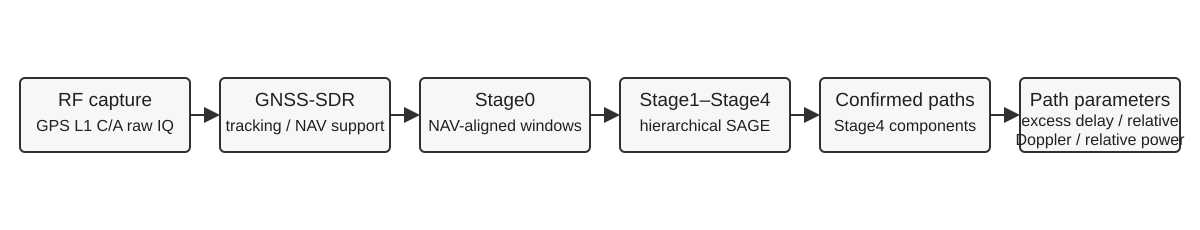
\includegraphics[width=\textwidth]{../../figures/figure1_workflow.pdf}
\caption{测量与处理流程：从动态射频捕获，经跟踪和 NAV 解码，到 NAV 对齐观测形成、候选筛选、时延—多普勒估计、时间验证、多快照确认和路径级参数。}
\label{fig:workflow-cn}
\end{figure*}

\section{导航信息辅助的层级式 SAGE 多径估计}
\subsection{信号与多径模型}
SAGE 估计遵循空间交替广义期望最大化（space-alternating generalized expectation-maximization）框架 \cite{fessler1994sage}，以及该方法在移动无线信道高分辨率参数估计中的既有应用 \cite{fleury1999sage}。接收复基带信号表示为
\begin{equation}
r(t)=s_0(t)+\sum_{\ell=1}^{L}\alpha_\ell s(t-\tau_\ell)\exp\!\left(j2\pi\Delta f_\ell t\right)+n(t),
\end{equation}
其中，$s_0(t)$ 表示直达分量；每个附加分量具有复增益 $\alpha_\ell$、时延 $\tau_\ell$ 和相对于直达分量的多普勒偏移 $\Delta f_\ell$。复增益包含幅度和相位。

\subsection{基于 SAGE 的时延—多普勒参数估计}
对于第 $i$ 次迭代中的第 $\ell$ 条路径，代码先从观测中减去其他路径的当前合成贡献，形成隐藏信号
\begin{equation}
r_\ell^{(i)}(t)=r(t)-\sum_{k\ne\ell}\hat{\alpha}_k^{(i)}q(t;\hat{\tau}_k^{(i)},\hat{\Delta f}_k^{(i)}),
\end{equation}
其中 $q(\cdot)$ 为带分数时延和多普勒的码复制。随后以归一化时延—多普勒相关目标细化当前路径：
\begin{equation}
(\hat{\tau}_\ell,\hat{\Delta f}_\ell)=\mathop{\arg\max}_{\tau,\Delta f}
\frac{|q(\tau,\Delta f)^{H}r_\ell^{(i)}|^2}{q(\tau,\Delta f)^{H}q(\tau,\Delta f)}.
\end{equation}
粗网格相关由 FFT/IFFT 实现，局部细化使用显式分数时延复制；随后通过当前复制矩阵的最小二乘求解更新复增益。最多迭代 10 次，或当残差 RSS 的相对变化低于 $10^{-6}$ 时停止。局部 SAGE 时延网格步长为 0.1 sample（0.01 chip），邻域半宽为 0.8 sample；局部多普勒范围为相对跟踪估计的 $\pm30$ Hz，步长为 5 Hz。

\subsection{NAV 辅助的观测形成}
特定通道的跟踪和遥测信息提供同步与样本支持。解码后的导航符号提供与 PRN 和时间对齐的符号序列，用于 NAV 擦除和完整 40 ms 观测窗口构造；PRN/通道关联用于选择目标跟踪信号流。由此形成的有效观测构成后续估计的母集，但该步骤不分配多径标签。在 10.23 MHz 下，采样与 C/A 码片的关系为每码片 10 个样本。

\subsection{候选筛选与局部模型阶数估计}
候选窗口筛选使用 $\pm125$ Hz、25 Hz 步长的主多普勒搜索、局部相关细化，以及受跟踪得到的相对多普勒界约束的残差搜索。筛选结果缩小了进入高成本局部 SAGE 拟合的窗口集合。对每个筛选窗口评估 $L=1,2,3,4$ 的分数时延—多普勒模型。阶数逐级增加必须满足模型有效、BIC 增益至少为 10 且增量 RSS 降低至少为 0.002\%。较高模型阶数表明引入额外信号分量能够改善局部观测的模型表示，而最终路径确认还需满足时间一致性和多快照联合验证。

\subsection{时间一致性与多快照联合确认}
时间验证在相邻窗口之间比较路径时延、多普勒和相对功率。可靠中心需要在半径 2 的窗口范围内形成至少 3 个连续匹配窗口，容差分别为 1.5 samples、40 Hz 和 10 dB。随后以可靠窗口为中心，对连续的 5 个 20 ms 快照进行约 100 ms 的联合估计。联合模型选择使用相同的顺序 BIC 规则，并要求高阶模型至少赢得 4 个快照。只有有效的联合解包含次级路径且满足联合确认路径表条件时，才进入确认集合；局部高阶选择和时间可靠中心仍属于中间证据。

以直达分量（$\ell=0$）为参考，路径 $\ell$ 的超额时延定义为 $\Delta\tau_\ell=\tau_\ell-\tau_0$，主要以 samples 表示；chip 数值由单位换算得到。相对多普勒（$\Delta f_\ell$）表示相对于直达分量的多普勒偏移，而不是绝对载波多普勒；相对功率以直达分量为参考。上述参数用于表征所评估环境中的已确认传播路径。

\section{实验结果}
\subsection{层级式路径提取行为}
为表征候选分量在处理链中的逐步收敛过程，本文总结了有效的 40 ms 观测窗口、候选窗口、时间一致候选以及最终联合确认结果。图~\ref{fig:hierarchical-confirmation-cn} 给出了三个代表性案例的候选缩减过程。对于每个候选窗口，局部 SAGE 估计分别评估 $L=1$--$4$ 的模型阶数；因此，这些评估表示同一窗口的不同模型阶数，而不是一组额外的独立观测。在 reference scene 的 G28 轨迹中，一个保持时间一致的候选随后被多快照联合确认排除。在 F1023\_V70\_D0120\_P1 场景的 G18 轨迹中，最终联合确认后没有候选保留为已确认多径事件。这些代表性案例用于说明层级式确认过程的行为；环境间的路径特征比较则基于表 II 和图 4 汇总的确认路径。该缩减过程体现了从局部表示、时间一致性到多快照联合确认逐步增强的证据要求。

\begin{table}[t]
\centering
\caption{不同动态车载环境下的测量覆盖与已确认多径路径。路径仅在联合确认准则下计数。}
\label{tab:experimental-evidence-cn}
\scriptsize
\setlength{\tabcolsep}{1pt}
\begin{tabular}{p{0.27\columnwidth}p{0.17\columnwidth}p{0.17\columnwidth}p{0.17\columnwidth}p{0.17\columnwidth}}
\toprule
环境 & \shortstack{独立\\场景数} & \shortstack{分析 PRN\\轨迹数} & \shortstack{已确认\\事件} & \shortstack{已确认\\路径}\\
\midrule
城市（Urban） & 4 & 4 & 7 & 7\\
山地/谷地（Mountain/Valley） & 3 & 9 & 13 & 14\\
高速/开阔（Highway/Open） & 2 & 2 & 2 & 2\\
特殊反射（Special Reflective） & 2 & 2 & 7 & 7\\
\bottomrule
\end{tabular}
\end{table}

\subsection{代表性 SAGE 提取多径案例}
图~\ref{fig:representative-path-cn} 展示来自高速/开阔场景的代表性 G25 测量。保留的联合确认路径具有 1.1 samples 的超额时延（次级路径时延为 1.2 samples）、$-4.7159$ Hz 的相对多普勒和 $-7.8526$ dB 的相对功率；其观测时间约为 60.5369 s，选择的模型阶数为 $L=2$。该案例展示了联合确认后直达传播分量与次级传播分量在时延、相对多普勒和相对功率上的可分离性。

\begin{figure}[t]
\centering
\includegraphics[width=\columnwidth]{../../figures/figure2_representative_path.pdf}
\caption{来自高速/开阔场景的代表性已确认 G25 路径。图中展示直达和次级分量及其超额时延、相对多普勒和相对功率。}
\label{fig:representative-path-cn}
\end{figure}

\begin{figure}[!t]
\centering
\includegraphics[width=\columnwidth]{../../figures/figure3_hierarchical_confirmation.pdf}
\caption{三个代表性测量案例中，从有效 40 ms 观测窗口经候选筛选、时间一致性和多快照联合确认到已确认路径的层级式缩减。该图用于说明处理层级中的确认行为。}
\label{fig:hierarchical-confirmation-cn}
\end{figure}

\subsection{环境级路径特征}
已确认路径集合包含来自 8 个独立场景、12 条包含已确认路径的 PRN 分析轨迹的 30 条路径观测；表 II 汇总了分析覆盖情况，其中也包括最终未形成确认路径的有效轨迹。所有已确认路径观测中，超额时延范围为 1.0--4.5 samples，有符号相对多普勒范围为 $-78.552$ 至 $49.664$ Hz，相对功率范围为 $-19.773$ 至 $-0.894$ dB。当前观测路径的 Urban、Mountain/Valley、Highway/Open 和 Special Reflective 超额时延中位数分别为 1.20、1.10、1.15 和 1.20 samples；相应的有符号相对多普勒中位数分别为 $-3.820$、$-0.468$、$-7.715$ 和 $31.540$ Hz。图 4 展示这三个共同可用的路径参数及其环境内中位数。

由首个和最后一个有效窗口推导、并对分析轨迹求和的观测跨度分别为 Urban 177.38 s、Mountain/Valley 203.16 s、Highway/Open 383.98 s 和 Special Reflective 150.50 s。这些时长用于说明各环境的实际观测范围。由于有效观测窗口存在重叠，事件数量用于概括观测到的确认案例，而不作为归一化发生率指标。

\begin{figure*}[!t]
\centering
\includegraphics[width=0.92\textwidth]{../../figures/figure4_environment_path_characteristics.pdf}
\caption{联合确认路径的环境级特征。各面板展示单条路径的超额时延、相对功率和有符号相对多普勒；标签给出各环境的样本数 $n$，横线表示环境内中位数。}
\label{fig:path-characteristics-cn}
\end{figure*}

\subsection{跨环境多径特征}
不同动态车载环境中观测到的多径参数呈现出不同的特征。Urban 测量具有当前数据中最宽的超额时延范围，最大超额时延达到 4.5 samples，表明实测信号中存在相对路径长度差异更大的反射分量。Mountain/Valley 获得的确认路径最多，并呈现较宽的相对多普勒变化范围，这与车辆运动下更丰富的时变传播几何定性一致。Special Reflective 在两个独立场景中均获得确认路径，其超额时延、相对功率和相对多普勒表现出较明显的变化范围，与局部强反射体条件定性一致。相比之下，当前可用的 Highway/Open 确认路径较少，其已观测时延和多普勒范围也较为集中。总体而言，这些实测差异与城市建筑、山地地形、开阔道路和局部反射体所对应的不同反射与散射条件定性一致，说明该框架能够从动态车载测量中分离并表征具有环境关联特征的多径行为。

\section{结论}
本文评估了一条真实动态 GPS L1 C/A 原始 IQ 测量链，以及一个用于路径级多径提取的导航信息辅助层级式 SAGE 框架。该估计器结合路径级时延—多普勒细化、NAV 对齐观测、时间一致性和多快照联合确认。现有证据支持对所测车载环境中的超额时延、相对多普勒和相对功率进行有界比较。未来工作将扩大独立场景覆盖，并建立更广泛统计分析所需的路径和信道参数数据库。

\bibliographystyle{IEEEtran}
\bibliography{../latex/references}

\end{document}
